% *********************************************************************
% © 2021-2023 Jeremy Sylvestre
%
% Permission is granted to copy, distribute and/or modify this document
% under the terms of the GNU Free Documentation License, Version 1.3 or
% any later version published by the Free Software Foundation; with no
% Invariant Sections, no Front-Cover Texts, and no Back-Cover Texts. A
% copy of the license is included in the appendix entitled “GNU Free
% Documentation License” that appears in the output document of this
% PreTeXt source code. All trademarks™ are the registered® marks of
% their respective owners.
%
% *********************************************************************

\newcommand*{\xmin}{0}
\newcommand*{\xmax}{4}
\newcommand*{\ymin}{0}
\newcommand*{\ymax}{3.75}

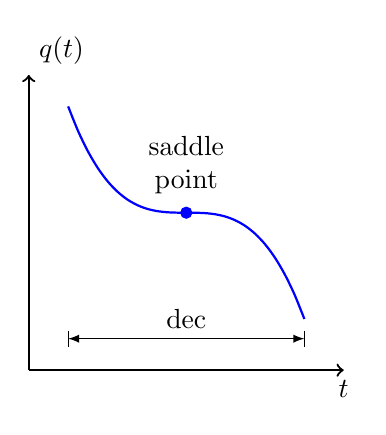
\begin{tikzpicture}
[
	closedpt/.style={circle,draw,fill,inner sep=0pt,minimum size=4pt},
	openpt/.style={circle,draw,inner sep=0pt,minimum size=4pt}
	% yscale=1.25
]

	% axes
	\draw[->,thick] (\xmin,0) -- (\xmax,0) node[below] {$t$};
	\draw[->,thick] (0,\ymin) -- (0,\ymax) node[above right] {$q(t)$};

	\draw[blue,thick,domain=0.5:3.5,smooth] plot (\x,{2 + (2 - \x)^3 / 2.5});

	\node[blue,closedpt] at (2,2) {};
	\node[align=center] at (2,2.6) {saddle\\point};

	\begin{scope}[yshift=-0.5cm]
	\draw
	  (0.5,1) -- (0.5,0.8)
	  (3.5,1) -- (3.5,0.8)
	;
	\draw[latex-latex] (0.5,0.9) -- (3.5,0.9);

	\node[above] at (2,0.9) {dec};

	\end{scope}

\end{tikzpicture}
